\section{Experiments}
\label{sec:Experiments}




\begin{figure}
\centering  
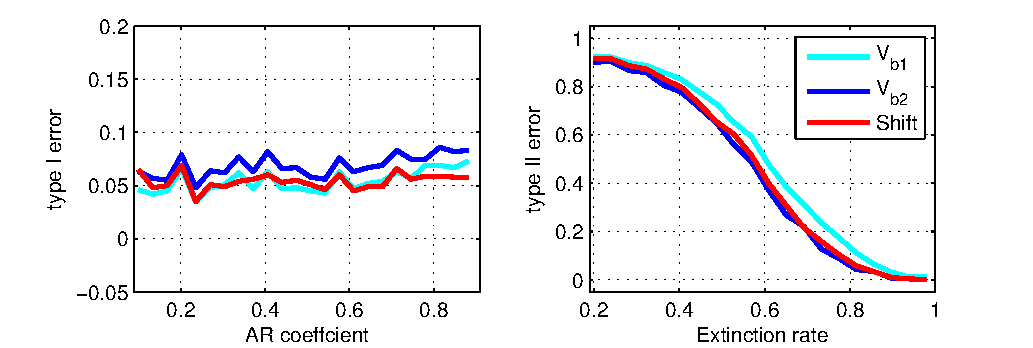
\includegraphics[width=1\textwidth]{arExtinct.pdf}
\caption{Comparison of Shift-HSIC and tests based on $V_{b1}$ and $V_{b2}$. Left panel show the performance under the null hypothesis, larger AR component implies a stronger temporal dependence. Right panel show the performance under the alternative hypothesis, larger extinction rate implies a greater dependence between processes.}
\label{fig:arExtinct}
\end{figure}

\begin{figure}
\centering  
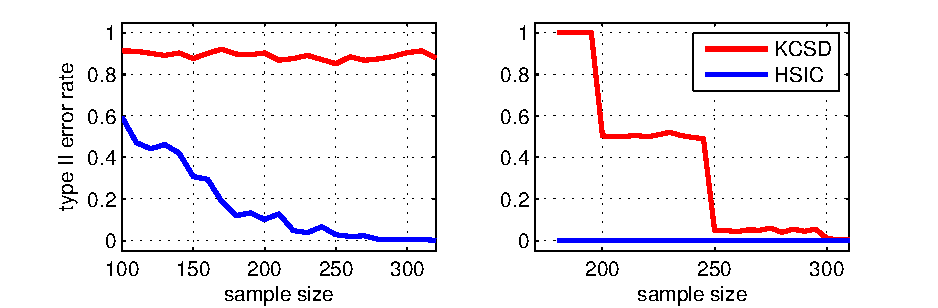
\includegraphics[width=1\textwidth]{varAndPhase.pdf}
\caption{In both panel Type II error is plotted. The left panel presents error of the lag-HSIC and KCSD algorithms for process following dynamics given by the equation \eqref{eq:dynamics2}, whereas the errors for process with dynamics given by equation \eqref{eg:dymamics1a} and \eqref{eg:dymamics1b} are shown in the right panel. X axis is indexed by the time series length i.e. sample size.}
\label{fig:phaseAndVar}
\end{figure}

\vspace{-0.2cm}
\paragraph{The MCMC M.D.}
It is natural to use MMD in order to diagnose how far an MCMC chain is from its stationary distribution \cite[Section 5]{sejdinovic_KAMH}, 
by comparing the MCMC sample to a benchmark sample. However, a hypothesis test of whether the sampler has converged based on the standard permutation-based bootstrap leads to too many rejections of the null hypothesis, due to  dependence within the chain. Thus, one would require heavily thinned chains, which is wasteful of samples and computationally burdensome.
Our experiments indicate that the wild bootstrap approach allows consistent tests directly on the chains, as it attains a desired number of false positives.\\
To assess performance of the wild bootstrap in determining MCMC convergence, we consider the situation where samples $\{X_i\}$ and $\{Y_i\}$ are bivariate, and both have the identical marginal distribution given by an elongated normal
$P=\mathcal{N}\left(\left[\protect\begin{array}{cc}
0 & 0\protect\end{array}\right],\left[\protect\begin{array}{cc}
15.5 & 14.5\protect\\
14.5 & 15.5
\protect\end{array}\right]\right)$.
However, they could have arisen either as independent samples, or as outputs of the Gibbs sampler with stationary distribution $P$. 
Table \ref{tab:gibbs_mmd} shows the \emph{rejection rates} under the significance level $\alpha=0.05$. It is clear that in the case where at least one of the samples is a Gibbs chain, the permutation-based test has a Type I error much larger than $\alpha$. 
The wild bootstrap using $V_{b1}$ (without artificial degeneration) yields the correct Type I error control in these cases. Consistent with findings in \cite[Section 5]{leucht_dependent_2013}, $V_{b1}$ mimics the null distribution better than $V_{b2}$. The bootstrapped statistic $\widehat{\text{MMD}}_{k,b}$ in \eqref{eq:mmdkb} which also relies on the artificially degenerated bootstrap processes, behaves similarly to $V_{b2}$.
In the alternative scenario where $\{Y_i\}$ was taken from a distribution with the same covariance structure but with the mean set to $\mu= \left[\protect\begin{array}{cc}
2.5 & 0\protect\end{array}\right]$, the Type II error for all tests was zero.
\vspace{-0.2cm}
\paragraph{Pitch-evoking sounds}
Our second experiment  is a two sample test on sounds studied in the field of pitch perception \cite{hehrmannthesis}. We synthesise the sounds with the fundamental frequency
parameter of treble C, subsampled at 10.46kHz. Each $i$-th period
of length $\Omega$ contains $d=20$ audio samples at times $0=t_{1}<\ldots<t_{d}<\Omega$
-- we treat this whole vector as a single observation $X_{i}$ or
$Y_{i}$, i.e., we are comparing distributions on $\mathbb{R}^{20}$.
Sounds are generated based on the AR process $a_{i}=\lambda a_{i-1}+\sqrt{1-\lambda^{2}}\epsilon_{i}$,
where $a_{0},\epsilon_{i}\sim\mathcal{N}(0,I_{d})$, with $X_{i,r}=\sum_{j}\sum_{s=1}^{d}a_{j,s}\exp\left(-\frac{\left(t_{r}-t_{s}-(j-i)\Omega\right)^{2}}{2\sigma^{2}}\right)$.
Thus, a given pattern -- a smoothed version of $a_{0}$ -- slowly
varies, and hence the sound deviates from
periodicity, but still evokes a pitch. We take
$X$ with $\sigma=0.1\Omega$
and $\lambda=0.8$, and $Y$ is either an independent copy of $X$
(null scenario), or has $\sigma=0.05\Omega$ (alternative scenario).%
\footnote{Such variation in the smoothness parameter changes the width of the
spectral envelope, i.e., the brightness of the sound.} $n_x$ is taken to be different from $n_y$. Results in Table \ref{tab:gibbs_mmd} demonstrate that the
approach using the wild bootstrapped statistic in \eqref{eq:mmdkb} allows control of the Type I error and reduction of the Type II error with the increasing sample size, while the permutation test
virtually always rejects the null hypothesis.
As in \cite{leucht_dependent_2013} and the MCMC example, the artificial degeneration of the wild bootstrap process causes the Type I error to remain above the design parameter of $0.05$, although it can be observed to drop with increasing sample size.

% \begin{table}
% \caption{Type I error for independent
% samples and Gibbs chains with identical marginal distributions; sample size=500, averaged over 200 trials. Wild bootstrap
% uses blocksize of $l_n=20$. A gaussian kernel with bandwidth
% $\sigma=1.7$ is used. Every second Gibbs sample is kept (i.e., after a pass
% through both dimensions).}
% \label{tab:gibbs_mmd}
% 
% \centering{}%
% \begin{tabular}{|c|c|c|c|c|}
% \hline 
% $X$ vs $Y$ & vanilla & $V_{b1}$ & $V_{b2}$ & $\widehat{\text{MMD}}_{k,b}$\tabularnewline
% \hline 
%  i.i.d. vs i.i.d.  & .040 & \textbf{.012}  & .070 & .025\tabularnewline
% \hline 
% i.i.d. vs Gibbs & .528  & \textbf{.052} & .105 & .100\tabularnewline
% \hline 
% Gibbs vs Gibbs & .680  & \textbf{.060} & .100 & .110\tabularnewline
% \hline 
% \end{tabular}
%\end{table}


\vspace{-0.2cm}
\paragraph{Instantaneous independence}
To examine instantaneous independence test performance, we compare it with the Shift-HSIC procedure \cite{chwialkowski2014kernel} on the 'Extinct Gaussian' autoregressive process proposed in the \cite[Section 4.1]{chwialkowski2014kernel}. Using exactly the same setting we compute type I error as a function of the temporal dependence and type II error as a function of extinction rate.\footnote{larger extinction rate implies a greater dependence between processes; larger AR component implies a stronger temporal dependence}  Figure \ref{fig:arExtinct} shows that all three tests (Shift-HSIC and tests based on $V_{b1}$ and $V_{b2}$) perform similarly.   
\vspace{-0.2cm}
\paragraph{Lag-HSIC}
The KCSD  \cite{besserve_statistical_2013} is, to our knowledge, the only test procedure to reject the null hypothesis if there exist $t$,$t'$ such that $Z_t$ and $Z_{t'}$ are dependent. In the experiments, we compare lag-HSIC with KCSD on two kinds of processes: one  inspired by econometrics and one from \cite{besserve_statistical_2013}.\\ 
In lag-HSIC, the number of lags under examination was equal to $\max\{10,\log n\}$, where $n$ is the sample size. We used Gaussian kernels with widths estimated by the median heuristic. The cumulative distribution of the $V$-statistics was approximated by samples from $n V_{b2}$. To model the tail of this distribution, we have fitted the generalized Pareto distribution to the bootstrapped samples (\cite{pickands1975statistical} shows that for a large class of underlying distribution functions such an approximation is valid).\\
The first process is a pair of two time series which share a common variance,   
\begin{align}
\label{eq:dynamics2}
 X_t = \epsilon_{1,k} \sigma_k^2, \quad  Y_t = \epsilon_{2,k}  \sigma_k^2,  \quad \sigma_k^2 = 1 + 0.45(X_t^2 + Y_t^2 ).
\end{align}
The above set of equations is an instance of the VEC dynamics \cite{bauwens_multivariate_2006} used in econometrics to model market volatility. The left panel of the Figure \ref{fig:phaseAndVar} presents the Type II error rate: for KCSD it remains at 90\% while for lag-HSIC it gradually drops to zero. The Type I error, which we calculated by sampling two independent copies $(X^{(1)}_{t},Y^{(1)}_{t})$ and $(X^{(2)}_{t},Y^{(2)}_{t})$ of the process and performing the tests on the pair $(X^{(1)}_{t},Y^{(2)}_{t})$, was around 5\% for both of the tests.\\
Our next experiment is a process sampled according to the dynamics proposed by \cite{besserve_statistical_2013},      
\begin{alignat}{2}
  \quad X_k &= \cos(\phi_{k,1})   &\quad  \phi_{k,1} &= \phi_{k-1,1} + 0.1\epsilon_{1,k} + 2 \pi f_1 T_s \label{eg:dymamics1a} \\  
  Y_k &= [2+C\sin(\phi_{k,1})]\cos(\phi_{k,2})  &   \phi_{k,2} &= \phi_{k-1,2} + 0.1\epsilon_{2,k} + 2 \pi f_2 T_s \label{eg:dymamics1b}
\end{alignat}
with parameters $C=.4$, $f_1=4Hz$,$f_2=20Hz$, and frequency $\frac {1} {T_s} = 100 Hz$. We compared performance of the KCSD algorithm, with parameters set to vales recommended in \cite{besserve_statistical_2013}, and the lag-HSIC algorithm. The Type II error of lag-HSIC, presented in the right panel of the Figure \ref{fig:phaseAndVar}, is substantially lower than that of KCSD. The Type I error ($C=0$) is equal or lower than 5\% for both procedures. Most oddly, KCSD error seems to converge to zero in steps. This may be due to the method relying on a spectral decomposition of the signals across a fixed set of bands. As the number of samples increases, the quality of the spectrogram will improve, and dependence will become apparent in bands where it was undetectable at shorter signal lengths.
 
